% This work is licensed under the Creative Commons
% Attribution-NonCommercial 3.0 Unported License. To view a copy of this
% license, visit http://creativecommons.org/licenses/by-nc/3.0/.

\section{Theorie}

\begin{figure}
  \centering
  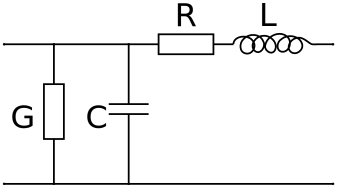
\includegraphics[scale=0.6]{ersatzschaltung}
  \caption{%
    Ersatzschaltung eines Koaxialkabels zwischen $x$ und $x + \d x$.
    Die Größen $R, L, G, C$ heißen Leitungskonstanten oder
    Leitungsbeläge.  Bei einer verlustfreien Leitung ist $R = G = 0$.
    Durch eine Betrachtung dieser Ersatzschaltung kann die
    Telegraphengleichung hergeleitet werden.}
  \label{fig:ersatz}
\end{figure}

Die Beschreibung der Ausbreitung von Signalen auf Leitungen ist
Gegenstand der Leitungstheorie.  Eine Leitung (zum Beispiel eine
Koaxialleitung, die in diesem Versuch verwendet wird) kann durch zwei
parallel verlaufende Leiter modelliert werden.  Grundaufgabe der
Leitungstheorie ist es, den zeitlichen Verlauf von Stromstärke $I(t, x)$
und Spannung $U(t, x)$ an jedem Ort $x$ der Leitung zu bestimmen.

Dazu wird ein Leitungstück von $x$ nach $x + \d x$ durch die
Ersatzschaltung aus Abbildung~\ref{fig:ersatz} dargestellt.  Die
Leitungsbeläge $R, L, G, C$ heißen auch Leitungskonstanten: $L$ und $C$
heißen Induktivitäts- bzw. Kapazitätsbelag, $R$ und $G$ heißen ohmscher
Belag bzw. Querleitfähigkeitsbelag.  Die beiden letzten kommen durch die
endliche Leitfähigkeit des Leitermaterials (Längsspannungsverluste) und
dielektrische Verlustströme zwischen der Isolierung der beiden Leiter
zustande.  Zwischen den Leitungsbelägen gibt es folgenden Zusammenhang:
%
\begin{equation}
  \label{eq:belagsformel}
  G = \frac{RC}{L}
\end{equation}

\subsection{Telegraphengleichung}

Im allgemeinen ergibt sich durch Betrachtung der Ersatzschaltung ein
System gekoppelter partieller Differentialgln. für $U$ und $I$.  Im
Falle konstanter Beläge kann dieses entkoppelt werden und es folgt eine
verallgemeinerte Wellengleichung:
%
\begin{equation}
  \label{eq:wellengl.}
  \pdn{2}{U}{x} - LC \pdn{2}{U}{t} = (LG+RC) \pd{U}{t} + RGU
\end{equation}
%
Diese Gleichung wird auch oft als Telegraphengleichung bezeichnet.  Die
Lösungen sind gedämpfte, hin- und rücklaufende harmonische Wellen:
%
\begin{equation}
  \label{eq:loesung}
  U(t, x) = U_0 \,e^{\iunt\omega t \pm \gamma x}
\end{equation}
%
Der Faktor $\gamma = \alpha + \iunt \beta = \sqrt{(R+\iunt \omega L)(G +
  \iunt \omega C)}$ heißt Ausbreitungskonstante, $\alpha$ heißt
Dämpfungsbelag und $\beta$ heißt Phasenbelag.  Die Phasengeschwindigkeit
der Welle ist daher frequenzabhängig und führt zu einer Verzerrung des
Signals.

\subsection{Leitungswellenwiderstand}

Die Art der Verzerrung wird vom Leitungswellenwiderstand beeinflußt,
welcher durch das Verhältnis von Strom- und Spannungswellen, die sich in
eine gemeinsame Richtung ausbreiten, bestimmt ist.  Für ein
sinusförmiges Signal mit der Frequenz $\omega$ ist der Wellenwiderstand
daher
%
\begin{equation}
  \label{eq:wellenwiderstand}
  Z_0 = \frac{U(\omega)}{I(\omega)} = \sqrt{\frac{R + \iunt \omega
      L}{G + \iunt \omega C}}\:.
\end{equation}
%

\subsection{Spannungs- und Strompulse}

In der Digital- und Nachrichtentechnik haben die Signale, die über eine
Leitung übertragen werden, oft die Form eines Pulses.  Die Lösungen der
entsprechenden Telegraphengleichung haben dann die Form eines hin- und
rücklaufenden Pulses, der durch die Reflexion am Leitungsende entsteht.
Der Quotient
%
\begin{equation}
  \Gamma = \frac{U_\text{r}}{U_0} = \frac{Z_\text{L} - Z_0}{Z_\text{L} + Z_0}
\end{equation}
%
heißt Reflexionsfaktor, wobei $Z_L$ hier die Lastimpedanz am Verbraucher
darstellt.  Mit seiner Hilfe kann die Form der rücklaufenden Welle aus
dem Eingangspuls berechnet werden.  Dazu wird die
\name{Laplace}-Transformation verwendet.  Sei nämlich $\tilde{U}_0(s)$
die \name{Laplace}-Transformierte der Spannung des einlaufenden und
$\tilde{U}_\text{r}(s)$ die \name{Laplace}-Transformierte der Spannung
des reflektierten Signals am Ort $x$ zur Zeit $t$, dann gilt
%
\begin{equation}
  \label{eq:reflex}
  \tilde{U}_\text{r}(s) = \Gamma\, \tilde{U}_0(s).
\end{equation}
%
Aus der Umkehrung dieser Formel unter Ausnutzung der inversen
\name{Laplace}-Transformation der zeitliche Verlauf der Spannung
$U_\text{r}(t, x)$ bestimmt werden.  Je nach Leitungsabschluß ergeben
sich hier verschiedene Signalformen.  Im Fall $Z_\text{L} = Z_0$ liegt
die sogenannte Leitungsanpassung vor, d.\,h. der Reflexionsfaktor
$\Gamma = 0$ und es gibt keine reflektierte Welle.

\subsection{Mehrfachreflexionen}

Ein Signal, das durch die Leitung läuft, wird nicht nur am Ende der
Leitung reflektiert, sondern auch am Anfang, wenn der Reflex wieder dort
ankommt.  So ergibt sich eine Reihe von Mehrfachreflexionen zwischen den
Kabelenden.  Bei jedem Reflex wird die Amplitude des Signals um einen
entsprechenden Reflexionsfaktor $\Gamma$ geschwächt.  Sei der
Reflexionsfaktor des Kabelanfangs $\Gamma_\text{a}$ und der des
Kabelendes $\Gamma_\text{e}$, dann gilt im Grenzfall unendlicher
Reflexion für die Amplitude der Signalspannung:
%
\begin{equation}
  U_\infty = U_0(1 + \Gamma_\text{e} + \Gamma_\text{a} \Gamma_\text{e}
  + \Gamma_\text{a} \Gamma_\text{e}^2 + \Gamma_\text{a}^2
  \Gamma_\text{e}^2 + \dotsb) = U_0 \:\frac{1 + \Gamma_\text{e}}{1
    - \Gamma_\text{a} \Gamma_\text{e}}
\end{equation}
%

Befinden sich im Kabel zusätzlich Störstellen (z.\,B. wenn zwei
verschiedene Kabel aneinander gesteckt sind), gibt es auch an diesen
Stellen Reflexionen.  Um den Überblick zu behalten, kann es in solchen
Fällen hilfreich sein, einen sogenannten Impulsfahrplan anzufertigen.
In Abschnitt~\ref{sec:durchfuehrung-mehrfachreflexion} wird eine
Situationen, in der zwei unterschiedliche Kabel verbunden sind,
beschrieben.

\subsection{Ausgewählte Leitungsabschlüsse}

In diesem Abschnitt werden die Signalverläufe zu drei verschiedenen
Abschlußwiderständen berechnet.  Die erhaltenen Funktionen werden später
verwendet, um eine Ausgleichsrechnung mit den aufgenommenen Meßwerten
durchzuführen.  Der einlaufende Signalverlauf\footnote{Die Amplitude
  wird hier auf 1 normiert, um die Rechnungen nicht zu überladen.  Da
  die \name{Laplace}-Transformation eine lineare Abbildung ist, kann ein
  Faktor für die Amplitude nachträglich hinzugefügt werden.}  kann mit
der \name{Heaviside}-Funktion~$\Theta$ so geschrieben werden:
%
\begin{equation}
  U_0(t) = \Theta(t).
\end{equation}
%
Die \name{Laplace}-Transformierte lautet dann $\tilde{U}_0(s) = s^{-1}$.
Mit Formel~\eqref{eq:reflex} wird daraus durch Rücktransformation der
Reflex am Leitungsende berechnet.

\paragraph{Abschluß durch Induktivität} Im Falle einer Induktivität als
Abschluß ist $Z_\text{L} = \iunt\omega L$ und damit ergibt sich für $s =
\iunt\omega$ der Reflexionsfaktor zu
%
\begin{equation}
  \Gamma = \frac{sL - Z_0}{sL + Z_0} = \frac{s - \tau^{-1}}{s + \tau^{-1}}
\end{equation}
%
mit $\tau := L/Z_0$. Jetzt wird gemäß Formel~\eqref{eq:reflex} das
reflektierte Signal berechnet.  Zerlege dazu $\Gamma \tilde{U}_0(s)$ in
Partialbrüche:
%
\begin{equation}
  \tilde{U}_\text{r}(s) = \Gamma\tilde{U}_0(s) = \frac{s - \tau^{-1}}{s(s
    + \tau^{-1})} = \frac{2}{s + \tau^{-1}} - \frac{1}{s}
\end{equation}
%
Nach den Eigenschaften der \name{Laplace}-Transformation bezüglich
Translation das reflektierte Signal für $t>0$ erhalten:
%
\begin{equation}
  \label{eq:ind_reflex}
  U_\text{r}(t) = 2e^{-\frac{t}{\tau}} - 1.
\end{equation}

\paragraph{Abschluß durch Induktivität und ohmschen Widerstand} In
diesem Fall wird $Z_\text{L} = R + \iunt \omega L$ und der
Reflexionsfaktor lautet
%
\begin{equation}
  \Gamma = \frac{R + sL - Z_0}{R + sL - Z_0} = \frac{s + (R-Z_0)L^{-1}}{s + \tau^{-1}}
\end{equation}
%
mit $\tau := L/(Z_0 + R)$.  Jetzt wird analog zu oben verfahren.  Eine
Partialbruchzerlegung von $\Gamma \tilde{U}_0(s)$ liefert:
%
\begin{equation}
  \tilde{U}_\text{r} (s) = \Gamma \tilde{U}_0(s) = \frac{s + (R -
    Z_0)L^{-1}}{s(s + \tau^{-1})} = \frac{\Gamma_0}{s} + \frac{1
    - \Gamma_0}{s + \tau^{-1}}
\end{equation}
%
mit $\Gamma_0 := \frac{R - Z_0}{R + Z_0}$.  Daraus wird das reflektierte
Signal durch Rücktransformation erhalten:
%
\begin{equation}
  \label{eq:ind_ohm_reflex}
  U_\text{r}(t) = \Gamma_0 + (1 - \Gamma_0) e^{-\frac{t}{\tau}}.
\end{equation}

\paragraph{Abschluß durch Kapazität und ohmschen Widerstand} Hier ist
$Z_\text{L} = R + \frac{1}{\iunt \omega C}$ und der Reflexionsfaktor
lautet dann:
%
\begin{equation}
  \Gamma = \frac{\frac{1}{sC} + R - Z_0}{\frac{1}{sC} + R + Z_0}
  = \frac{\Gamma_0 s + \tau^{-1}}{s + \tau^{-1}} 
\end{equation}
%
mit $\Gamma_0$ wie oben und $\tau := (R+Z_0) C$.  Nach der
Partialbruchzerlegung
%
\begin{equation}
  \Gamma \tilde{U}_0(s) = \frac{1}{s} + \frac{\Gamma_0 - 1}{s + \tau^{-1}}
\end{equation}
%
lautet nach Rücktransformation das reflektierte Signal so:
%
\begin{equation}
  \label{eq:cap_ohm_reflex}
  U_\text{r}(t) = 1 + (\Gamma_0 - 1) e^{-\frac{t}{\tau}}.
\end{equation}
